\documentclass[sigconf]{aamas} % Comment this line out if you need a4paper


\usepackage{amsmath, amssymb , graphicx}
\usepackage{multirow}
\usepackage{multicol}
\usepackage{siunitx}
\usepackage{color}
\usepackage{array}
\usepackage{makecell}
\usepackage{hyperref}
\hypersetup{colorlinks=true}
\usepackage{xargs}
\newcommand{\etal}{\textit{et~al}.}
%\usepackage{dblfloatfix} %thank you!!
\usepackage{booktabs}
\setlength{\marginparwidth}{2cm}
\usepackage[colorinlistoftodos,prependcaption,textsize=tiny]{todonotes}
\newcommandx{\unsure}[2][1=]{\todo[linecolor=red,backgroundcolor=red!25,bordercolor=red,#1]{#2}}
% \newcommandx{\change}[2][1=]{\todo[linecolor=blue,backgroundcolor=blue!25,bordercolor=blue,#1]{#2}}
% \newcommandx{\info}[2][1=]{\todo[linecolor=OliveGreen,backgroundcolor=OliveGreen!25,bordercolor=OliveGreen,#1]{#2}}
% \newcommandx{\improvement}[2][1=]{\todo[linecolor=Plum,backgroundcolor=Orange!25,bordercolor=Orange,#1]{#2}}

%\renewcommand{\cellalign/theadalign}{vh}
%\newcommand{\rpm}{\raisebox{.2ex}{$\scriptstyle\pm$}}

%\DeclareCaptionFont{caption}{\fontsize{8}{9.6}\selectfont}
%\captionsetup{font=caption}

\usepackage{hyperref}
\hypersetup{
    colorlinks=true,
    linkcolor=blue,
    filecolor=blue,      
    urlcolor=blue,
}

\urlstyle{same}

%\usepackage[usestackEOL]{stackengine}

\usepackage{subcaption}
\usepackage [english]{babel}
\usepackage [autostyle, english = american]{csquotes}
\MakeOuterQuote{"}\captionsetup{compatibility=false}

%% do not change the following lines
\usepackage{flushend}
\setcopyright{ifaamas}  % do not change this line!
\acmDOI{doi}  % do not change this line!
\acmISBN{}  % do not change this line!
\acmConference[AAMAS'20]{Proc.\@ of the 19th International Conference on Autonomous Agents and Multiagent Systems (AAMAS 2020), B.~An, N.~Yorke-Smith, A.~El~Fallah~Seghrouchni, G.~Sukthankar (eds.)}{May 2020}{Auckland, New Zealand}  % do not change this line!
\acmYear{2020}  % do not change this line!
\copyrightyear{2020}  % do not change this line!
\acmPrice{}  % do not change this line!

\usepackage{amsmath}
\usepackage{bbm}
%\newcommand{\TODO}[1]{}
\newcommand{\TODO}[1]{{\color{red}TODO: {#1}}}

\def\state{s}
\def\statet{\state_t}
\def\statetp{\state_{t-1}}
\def\statehist{\state_{1:t-1}}
\def\statetn{\state_{t+1}}
\def\obs{\meas}
\def\obst{\obs_t}
\def\act{a}
\newcommand{\ctrl}{u}
\def\actt{\act_t}
\def\acttp{\act_{t-1}}
\def\acttn{\act_{t+1}}
\def\Obs{\mathcal{O}}
\def\ObsEnc{\Phi_o}
\def\ObsProb{P_o}
\def\ObsFunc{C}
\def\ObsFuncFull{\ObsFunc(\statet, \actt) \rightarrow \obst}
\def\ObsFuncInv{\ObsFunc^{-1}}
\def\ObsFuncInvFull{\ObsFuncInv(\obst, \statetp, \actt) \rightarrow \statet}
\def\State{\mathcal{S}}
\def\Action{\mathcal{A}}
\newcommand{\CtrlSp}{\mathcal{U}}
\def\TransP{P_{T}}
\def\Trans{T}
\def\TransFull{\Trans(\statet, \actt) \rightarrow \statetn}
\def\TransObs{T_c}
\def\Rew{R}
\def\rew{r}
\newcommand{\vect}[1]{\mathbf{#1}}
\def\rewards{\vect{r}_{1:t}}
\def\rewt{\rew_t}
\def\rewtp{\rew_{t-1}}
\def\rewtn{\rew_{t+1}}
\def\RewFull{\Rew(\statet, \actt) \rightarrow \rewtn}
\def\TransObsFull{\TransObs(\statet, \obst, \actt, \rewt; \theta_T) \rightarrow \statetn}
\def\Value{V}
\def\pit{\pi_t}
\def\piDef{\pi(\acttn|\statet, \obst, \actt, \rewt; \theta_\pi) \rightarrow \pit(\acttn ; \theta_\pi)}
\def\Valuet{\Value_t}
\def\ValueDef{\Value(\statet, \obst, \actt, \rewt; \theta_\Value) \rightarrow \Valuet(\theta_\Value)}
\def\R{\mathbb{R}}
\def\E{\mathbb{E}}
\newcommand{\Goal}{\mathcal{G}}
\newcommand{\goalRV}{G}
\newcommand{\meas}{z}
\newcommand{\measurements}{\vect{\meas}_{1:t}}
\newcommand{\meast}[1][t]{\meas_{#1}}
\newcommand{\param}{\theta}
\newcommand{\policy}{\pi}
\newcommand{\graph}{G}
\newcommand{\vtces}{V}
\newcommand{\edges}{E}
\newcommand{\st}{\state}
\newcommand{\stn}{\st_{t+1}}
\newcommand{\stt}{\st_t}
\newcommand{\stk}{\st_k}
\newcommand{\stj}{\st_j}
\newcommand{\sti}{\st_i}
\newcommand{\St}{\mathcal{S}}
\newcommand{\Act}{\mathcal{A}}
\newcommand{\acti}{\act_i}
\newcommand{\lpt}{\delta}
\newcommand{\trans}{P_T}
\newcommand{\Q}{\qValue}
\newcommand{\V}{V}

\newcommand{\fwcost}{Q}
\newcommand{\fw}{\fwcost}
\newcommand{\qValue}{Q}
\newcommand{\prew}{\Upsilon}
\newcommand{\epiT}{T}
\newcommand{\vma}{\alpha_\Value}
\newcommand{\qma}{\alpha_\qValue}
\newcommand{\prewma}{\alpha_\prew}
\newcommand{\fwma}{\alpha_\fwcost}
\newcommand{\maxValueBeam}{\vect{\state}_{\Value:\text{max}(m)}}
\newcommand{\nil}{\emptyset}
\newcommand{\discount}{\gamma}
\newcommand{\minedgecost}{\fwcost_0}
\newcommand{\goal}{g}
\newcommand{\pos}{x}
%\newcommand{\fwargs}[5]{\fw_{#4}^{#5}\left({#3}\middle|{#1}, {#2}\right)}
\newcommand{\fwargs}[5]{\fw_{#4}^{#5}\left({#1}, {#2}, {#3}\right)}
\newcommand{\Rgoal}{R_{\text{goal}}}

\newcommand{\map}{m}
\newcommand{\MapSp}{\mathcal{M}}

\newcommand{\pose}{x}
\newcommand{\PoseSp}{\mathcal{X}}
\newcommand{\hpose}{\hat{\pose}}


\newcommand{\tgt}{y}
\newcommand{\TgtSp}{\mathcal{Y}}
\newcommand{\htgt}{\hat{\tgt}}
\newcommand{\btgt}{\bar{\tgt}}
\newcommand{\VarTgt}{\Sigma}

\newcommand{\rssi}{z}
\newcommand{\RSSI}{Z}
%\newcommand{\RSSISp}{\mathcal{Z}}
\newcommand{\RSSISp}{\R}
\newcommand{\RSSIModel}{\phi}

\newcommand{\hmap}{\hat{\map}}

\newcommand{\lidar}{l}
\newcommand{\LidarSp}{\mathcal{L}}
\newcommand{\LidarModel}{\psi}

\newcommand{\img}{I}
\newcommand{\ImgSp}{\mathcal{I}}
\newcommand{\ImgModel}{\chi}

\newcommand{\AlgSLAM}{\text{SLAM}}
\newcommand{\AlgObjDet}{\text{ObjDet}}
\newcommand{\AlgTgt}{\text{TgtEst}}

\newcommand{\cost}{c}

\newcommand{\dyn}{f}
\newcommand{\ind}{\mathbbm{1}}
\newcommand{\rnoise}{\epsilon}
\newcommand{\pnoise}{\eta}
\newcommand{\lnoise}{\omega}
\newcommand{\rCov}{R}
\newcommand{\pCov}{P}
\newcommand{\lCov}{L}

%\newtheorem{problem}{Problem}
\newcommand{\En}{\mathbb{H}}
\newcommand{\MI}{\mathbb{I}}
\newcommand{\bel}{\textit{bel}}

\newcommand{\N}{\mathcal{N}}
\newcommand{\mpose}{\bar{\pose}}
\newcommand{\SPose}{\Sigma}
\newcommand{\mtgt}{\bar{\tgt}}
\newcommand{\STgt}{\Xi}
\newcommand{\mask}{\chi}
\newcommand{\Data}{\mathcal{D}}
\let\svfootnoterule\footnoterule
\renewcommand\footnoterule{\vfill\svfootnoterule}

%IEEE
%\usepackage[redeflists]{IEEEtrantools}

\title{
  Source seeking with map prediction in partially observable environments
}

%\author{Paper 1842}  % put your paper number here!

\author{Carlos Nieto-Grandas$^\dagger$}
\author{Vikas Dhiman}%$^\dagger$}
\author{Henrik I. Christensen}% <-this % stops a space
\affiliation{%
  \institution{University of California, San Diego}
  %\streetaddress{9500 Gilman Drive}
  \city{$^\dagger$US Army Research Laboratory}
  %San Diego}
  %\state{California}
  \postcode{92121}}
\email{cnietogr,vdhiman,hic@ucsd.edu}%

\begin{document} 


%%%%%%%%%%%%%%%%%%%%%%%%%%%%%%%%%%%%%%%%%%%%%%%%%%%%%%%%%%%%%%%%%%%%%%
%abstract
\begin{abstract}
We focus on the problem of stochastic source seeking in partially observable
environments.
Robots being deployed in search and rescue scenarios often need to
seek the source of a signal, like radio-active material, heat signature or gas leakages.
However, this problem is accentuated in partially observable
environments.
One needs to know the map before planning an exploratory trajectory.
We address this problem by formulating map-prediction as an image inpainting
problem.
Using the predicted map, we plan a trajectory that maximizes the information
gain for the target locations.
\end{abstract}
\keywords{Active exploration; Robotics; partial observability}  % put your semicolon-separated keywords here!

\maketitle

%%%%%%%%%%%%%%%%%%%%%%%%%%%%%%%%%%%%%%%%%%%%%%%%%%%%%%%%%%%%%%%%%%%%%%
%
% \begin{IEEEkeywords}
% \textbf{Keywords: Semantic Scene Understanding, Mapping, Recognition.}
% \end{IEEEkeywords}

%%%%%%%%%%%%%%%%%%%%%%%%%%%%%%%%%%%%%%%%%%%%%%%%%%%%%%%%%%%%%%%%%%%%%%
%sections

\section{Introduction}\label{sec:intro}

Search and rescue robots often need to find source of a signal like radio-active material, heat signature or gas leak. 
This problem is known as stochastic source seeking.
To plan an optimal exploration trajectory, many researchers~\cite{atanasov2014StochasticSourceSeeking} have suggested using 
information gain metrics like Mutual Information.
However, in partially observable environments computing information gain of 
a trajectory becomes challenging if parts of map are unknown. 
We address this problem by predicting unknown maps as an image inpainting problem.

Stochastic source seeking has been typically addressed in fully
   observable environments, with a single target~\cite{atanasov2014StochasticSourceSeeking}.
   On the other hand, exploration in partially observable
   environment~\cite{choudhury2017adaptive} has dealt
   with exploration without a source seeking objective.
We show how existing approaches that depend upon fully observable state do
not generalize to all kind of maps and obstacles. 

%Specifically, we consider a U-maze (Fig~\ref{fig:c-maze}), which has local optima with respect to greedy source seeking.
The work closest to our approach is Shreshta~et~al.~\cite{shreshta2019icra}.
However, they attempt to predict large regions in the map which are unlikely to generalize to new maps.
Moreover, Shreshta~et~al.~\cite{shreshta2019icra} use a flood fill over the
predicted map to estimate the information gain for each action. 
Flood filling can be brittle and lead to misleading information gains with even small holes in the walls of the map.
Instead, we predict only the occupancy of the to be filled in the next few laser scans and the possible information gained next few steps.
Further, Shreshta~et~al.~\cite{shreshta2019icra} evaluate there algorithm on simple map exploration task. 
To the best of our knowledge, map prediction has not been yet applied to source seeking.

We extend the source seeking approaches to partially observable environments
while building the map of the environment. We learn priors over the maps of
indoor buildings and predict unknown parts of the maps using Generative
Adversarial Networks~\cite{goodfellow2014GAN}, specifically
DeepFill~\cite{yu2018DeepFill}. With the map-predictive abilities, we apply
standard techniques used for Mutual Information maximization when map is known.
We show how our approach overcomes the challenges introduced by the
\emph{C-Maze} (Fig~\ref{fig:c-maze}).

%
\begin{figure}%
  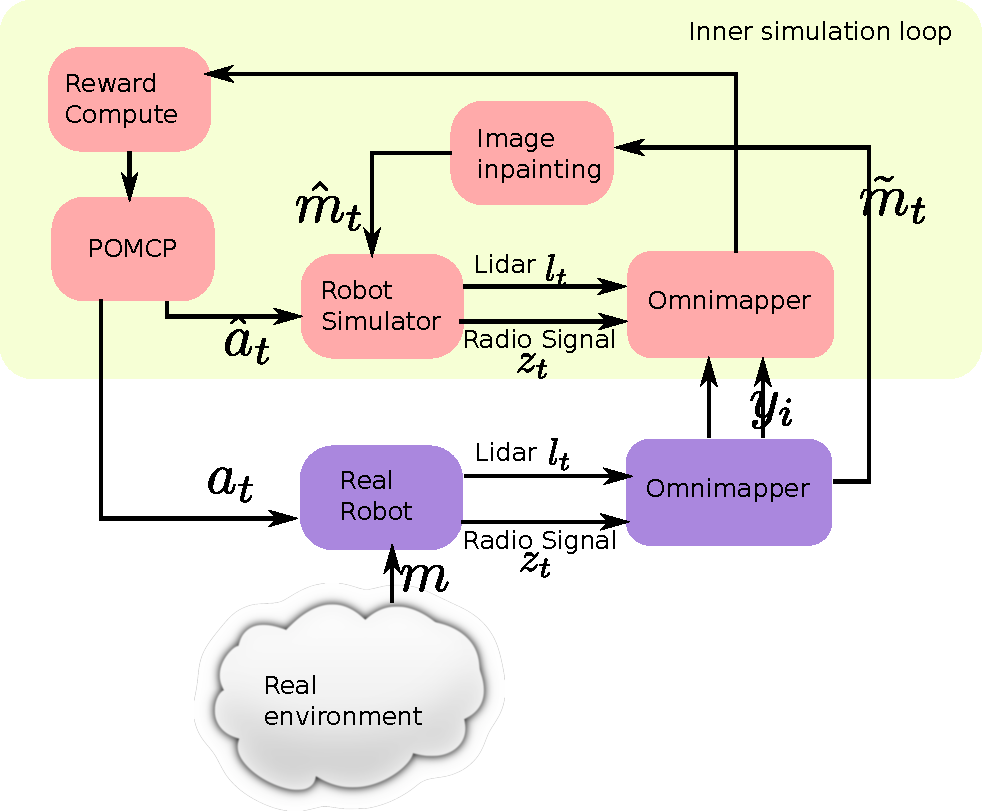
\includegraphics[width=\columnwidth]{files/media/overall-architecture.pdf}
  \caption{Overall architecture}%
  \label{fig:architecture}%
\end{figure}%
% 

%


\begin{figure*}
\parbox[][][b]{0.22\linewidth}{%
\centering 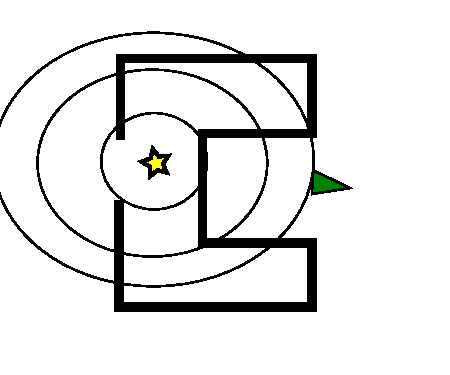
\includegraphics[width=\linewidth]{./files/media/u-maze.pdf}\\(a)}
\parbox[][][b]{0.27\linewidth}{%
\centering 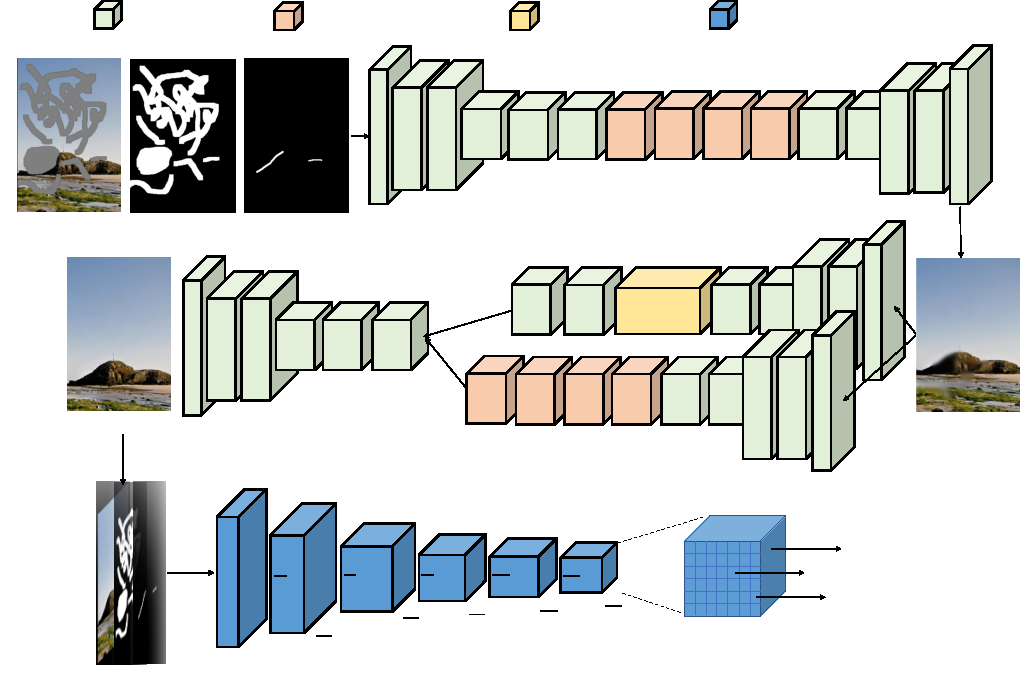
\includegraphics[width=\linewidth]{./files/media/deepfill-architecture.pdf}\\(b)}
\parbox[][][b]{0.24\linewidth}{%
\centering \includegraphics[width=\linewidth]{paper/files/media/atk_exploration.png}\\(c)}
\parbox[][][b]{0.24\linewidth}{%
\centering \includegraphics[width=\linewidth]{paper/files/media/zigxbee.png}\\(d)}
  \caption{
  (a) U-maze. If the green robot greedily follows the radio signal from the
  yellow target, then it is likely to get stuck in the local minima. Our
  algorithm has dual objective of exploration and source seeking. When the gain
  in source seeking is small then the robot reverts to environment exploration
  and escapes local minima.
  (b) DeepFill architecture. Image from \cite{yu2018DeepFill}
  (c) Our multi-robot team of jackal robots exploring Atkinson Hall's first floor getting measurements from ZigXbees transmitters. 
  (d) On the right a picture of the ZigXbee transmitter used on these experiments.}%
  \label{fig:exp:expl_atk}%
  \label{fig:deepfill}%
  \label{fig:c-maze}
\end{figure*}
\section{Background}

\subsection{Stochastic source seeking}
Stochastic source seeking is the problem of searching  a stochastic source
$\tgt_i \in \TgtSp$ of a signal in an unknown environment.
The problem of stochastic source seeking is typically addressed either using
model-based or model-free methods.
Model-based methods assume that the signal model
$\RSSIModel: \TgtSp \times \PoseSp \times \MapSp \rightarrow \RSSISp$
is given, such that noisy signal $\rssi_{i,t}$ at time $t$ with robot pose
$\pose_t \in \PoseSp$ , source position $\tgt_i \in \TgtSp$ and map $\map \in
\MapSp$ is given by
%
\begin{align}
\rssi_{i,t} &= \RSSIModel(\tgt_i, \pose_t, \map) + \rnoise_t,
\end{align}%
% 
where $\rnoise_t \sim  \N(0, \Sigma)$ is zero mean Gaussian noise.

On the other model-free methods assume that $\RSSIModel$ is unknown and usually
follow greedy signal-gradient based approach.

\begin{problem}[Model-based source seeking]
Consider $N$ targets, whose locations $\mathbf{\tgt} := (\tgt_i)_{i=1}^N$ are unknown. We are given
a robot with pose $\pose_t$ that moves according to a given dynamics model
$\pose_{t+1} = \dyn(\pose_t, \ctrl_t, \map) + \pnoise_t$. We want to find the
policy $\policy$ that maximizes the information gain about the target locations,
%
\begin{equation}\begin{split}
    \policy^* = \arg&\max_{\policy} \MI( \mathbf{\tgt}_{1:N} ; \rssi_{1:t} )
  \\
  \text{s.t } \quad
  \pose_{t+1} &= \dyn(\pose_t, \ctrl_t, \map) + \pnoise_t
  \\
  \rssi_{t} &= \sum_{i=1}^N \RSSIModel(\pose_t, \tgt_i, \map) + \rnoise_{i,t}
  \\
  \ctrl_t &= \policy(\rssi_{1:t})
\end{split}\end{equation}
%
\end{problem}


\subsection{Information gathering}

Information gathering is the problem of exploring an unknown environment with
the objective of collecting maximum information about the environment map. Given a robot with pose $\pose_t$ at time $t$ is present in an unknown
environment $\map$ and is observes lidar scans $\lidar_t = \LidarModel(\pose_t,
\map) + \lnoise_t$ according to a known observation model $\LidarModel$. Also
assume that the dynamics of the robot are known.
\begin{problem}[Information Gathering]
The Information Gathering
problem is the problem of seeking to maximizing the information about the unknown
map $\map$ using the observations $\lidar_{1:t}$,
%
\begin{equation}\begin{split}
      \policy^* = \arg&\min_{\policy} \En(\map \mid \lidar_{1:t}, \pose_{1:t})
      \\
      \text{s.t } \quad
  \pose_{t+1} &= \dyn(\pose_t, \ctrl_t, \map) + \pnoise_t
  \\
  \lidar_{t} &= \LidarModel(\pose_t, \map) + \lnoise_t
  \\
  \ctrl_t &= \policy(\lidar_{1:t}),
\end{split}\end{equation}
%
where $\En(\map \mid \lidar_{1:t}, \pose_{1:t})$ is an information measure over
the map $\map$. Typically it is the Shanon entropy of the map random variable.
\end{problem}

In this work, we combine the two problems and define the problem of stochastic
source seeking in partially observable environment.
% Consider the problem of active exploration, which seeks to find the optimal
% sequence of actions $\bfu$ that lead maximum gain in map-belief $\bel(\bfm)$
% information,
% \begin{equation}
% \begin{split}
%   \max_{\bfu_k} \sum_{t=k}^T &|\bbH(\bel(\bfm)_t) - \bbH(\bel_{t+1}(\bfm) | \bfx_t, \bfu_t)|
%   \\
%   \bfx_{t+1} &= f(\bfx_t, \bfu_t)
%   \\
%   \bfz_t &= g(\bfx_t)
%   \\
%   \bel_{t}(\bfm), \bfx_{t} &= \SLAM(\bel_{t-1}(\bfm), \bfx_{t-1}, \bfz_t, \bfu_t),
% \end{split}
% \end{equation}
% where $ \bel_t(\bfm) \triangleq \bbP(\bfm | \bfz_{1:t}, \bfu_{1:t})$ is the
% estimated map-belief at time $t$ or the probability of map given observations
% $\bfz_{1:t}$ up to time $t$.
% 
% This problem is understood to be intractable \TODO{citation needed}, hence only
% solved greedily.

We intend to capture the prior over map $\bbP(\bfm)$ using semantic patterns. Let the
map be composed of $n$ rooms $\bfr_i $, $\bfm = [\bfr_1; \dots; \bfr_n]$,
with respective semantic labels as $\bfc = [c_1; \dots; c_n]$.
Let the rooms be divided into a set of explored rooms $\bfm_e = \{ \bfr_e \mid
\exists t : \bfx_t \in \bfr_e \}$ and unexplored
rooms $\bfm_u = \{ \bfr_u \mid \forall t : \bfx_t \notin \bfr_u \}$, depending
upon whether the robot (position $\bfx_t$ ) has visited the room so far $\bfx_t
\in \bfr$.
We factorize the prior over map such that the observations $\bfz_{1:t}$ only
impact the estimation of explored rooms, while the unexplored rooms are only
based on prior,
\begin{align}
  \bbP(\bfm | \bfz_{1:t}, \bfu_{1:t}) = \bbP(\bfm_u | \bfm_e) \bbP(\bfm_e | \bfz_{1:t}, \bfu_{1:t}).
\end{align}
Here we assume that unexplored rooms $\bfm_u$ are independent of observations so
far, provided the explored rooms $ \bfm_u \perp \{ \bfz_{1:t}, \bfu_{1:t} \} | \bfm_e$.
To focus on capturing the semantic patterns, we further factorize the
conditional probability $\bbP(\bfm_u | \bfm_e)$ only through the corresponding
semantic labels of explored rooms $\bfc_e$ and unexplored rooms $\bfc_u$.
\begin{align}
  \bbP(\bfm_u | \bfm_e) &= \bbE_{\bfc_u, \bfc_e} \big[
  \bbP(\bfm_u | \bfc_u) \bbP(\bfc_u|\bfc_e) \bbP(\bfc_e | \bfm_e)
  \big].
\end{align}

This equation captures our basic assumption and in this work, we evaluate the
effectiveness of this assumption in exploration related tasks.

 %
\begin{figure*}[h!]%
  \def\frac{0.24}
  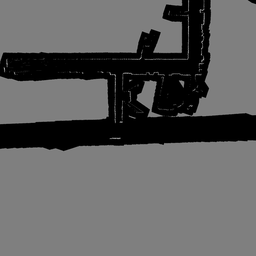
\includegraphics[width=\frac\linewidth]{./files/media/department_diiga/00016_input.png}%
  
\includegraphics[width=\frac\linewidth]{./files/media/department_diiga/00016_mask.png}%
  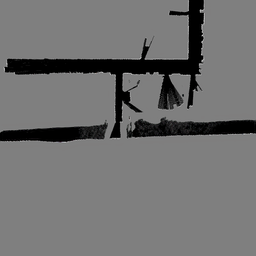
\includegraphics[width=\frac\linewidth]{./files/media/department_diiga/0016_output.png}%
  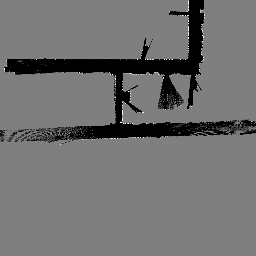
\includegraphics[width=\frac\linewidth]{./files/media/department_diiga/00016_estimated.png}%
  \\%
  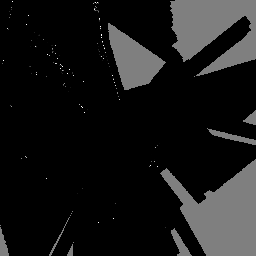
\includegraphics[width=\frac\linewidth]{./files/media/fr_campus_100p_10cm/00009_input.png}%
  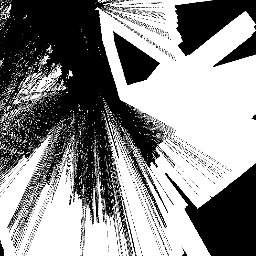
\includegraphics[width=\frac\linewidth]{./files/media/fr_campus_100p_10cm/00009_mask.png}%
  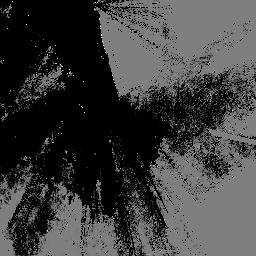
\includegraphics[width=\frac\linewidth]{./files/media/fr_campus_100p_10cm/00009_output.png}%
  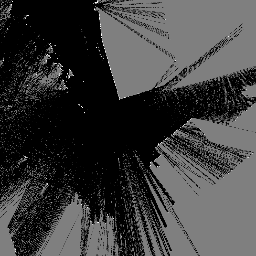
\includegraphics[width=\frac\linewidth]{./files/media/fr_campus_100p_10cm/00009_estimated.png}%
  \caption{Map prediction using DeepFill~\cite{yu2018DeepFill}. Given a map at
any timestep $\map_{t}$, we want to predict the map at $\map_{t+1}$. We create a
mask by morphological operations on the known area in $\map_t$. The resultant
mask is used to mark the regions that need to be predicted. The left column
shows the input map, the middle column shows the mask and the last column shows
the predicted map.}%
  \label{fig:map-prediction}%
\end{figure*}%

\begin{figure*}[h!]
 \centering
 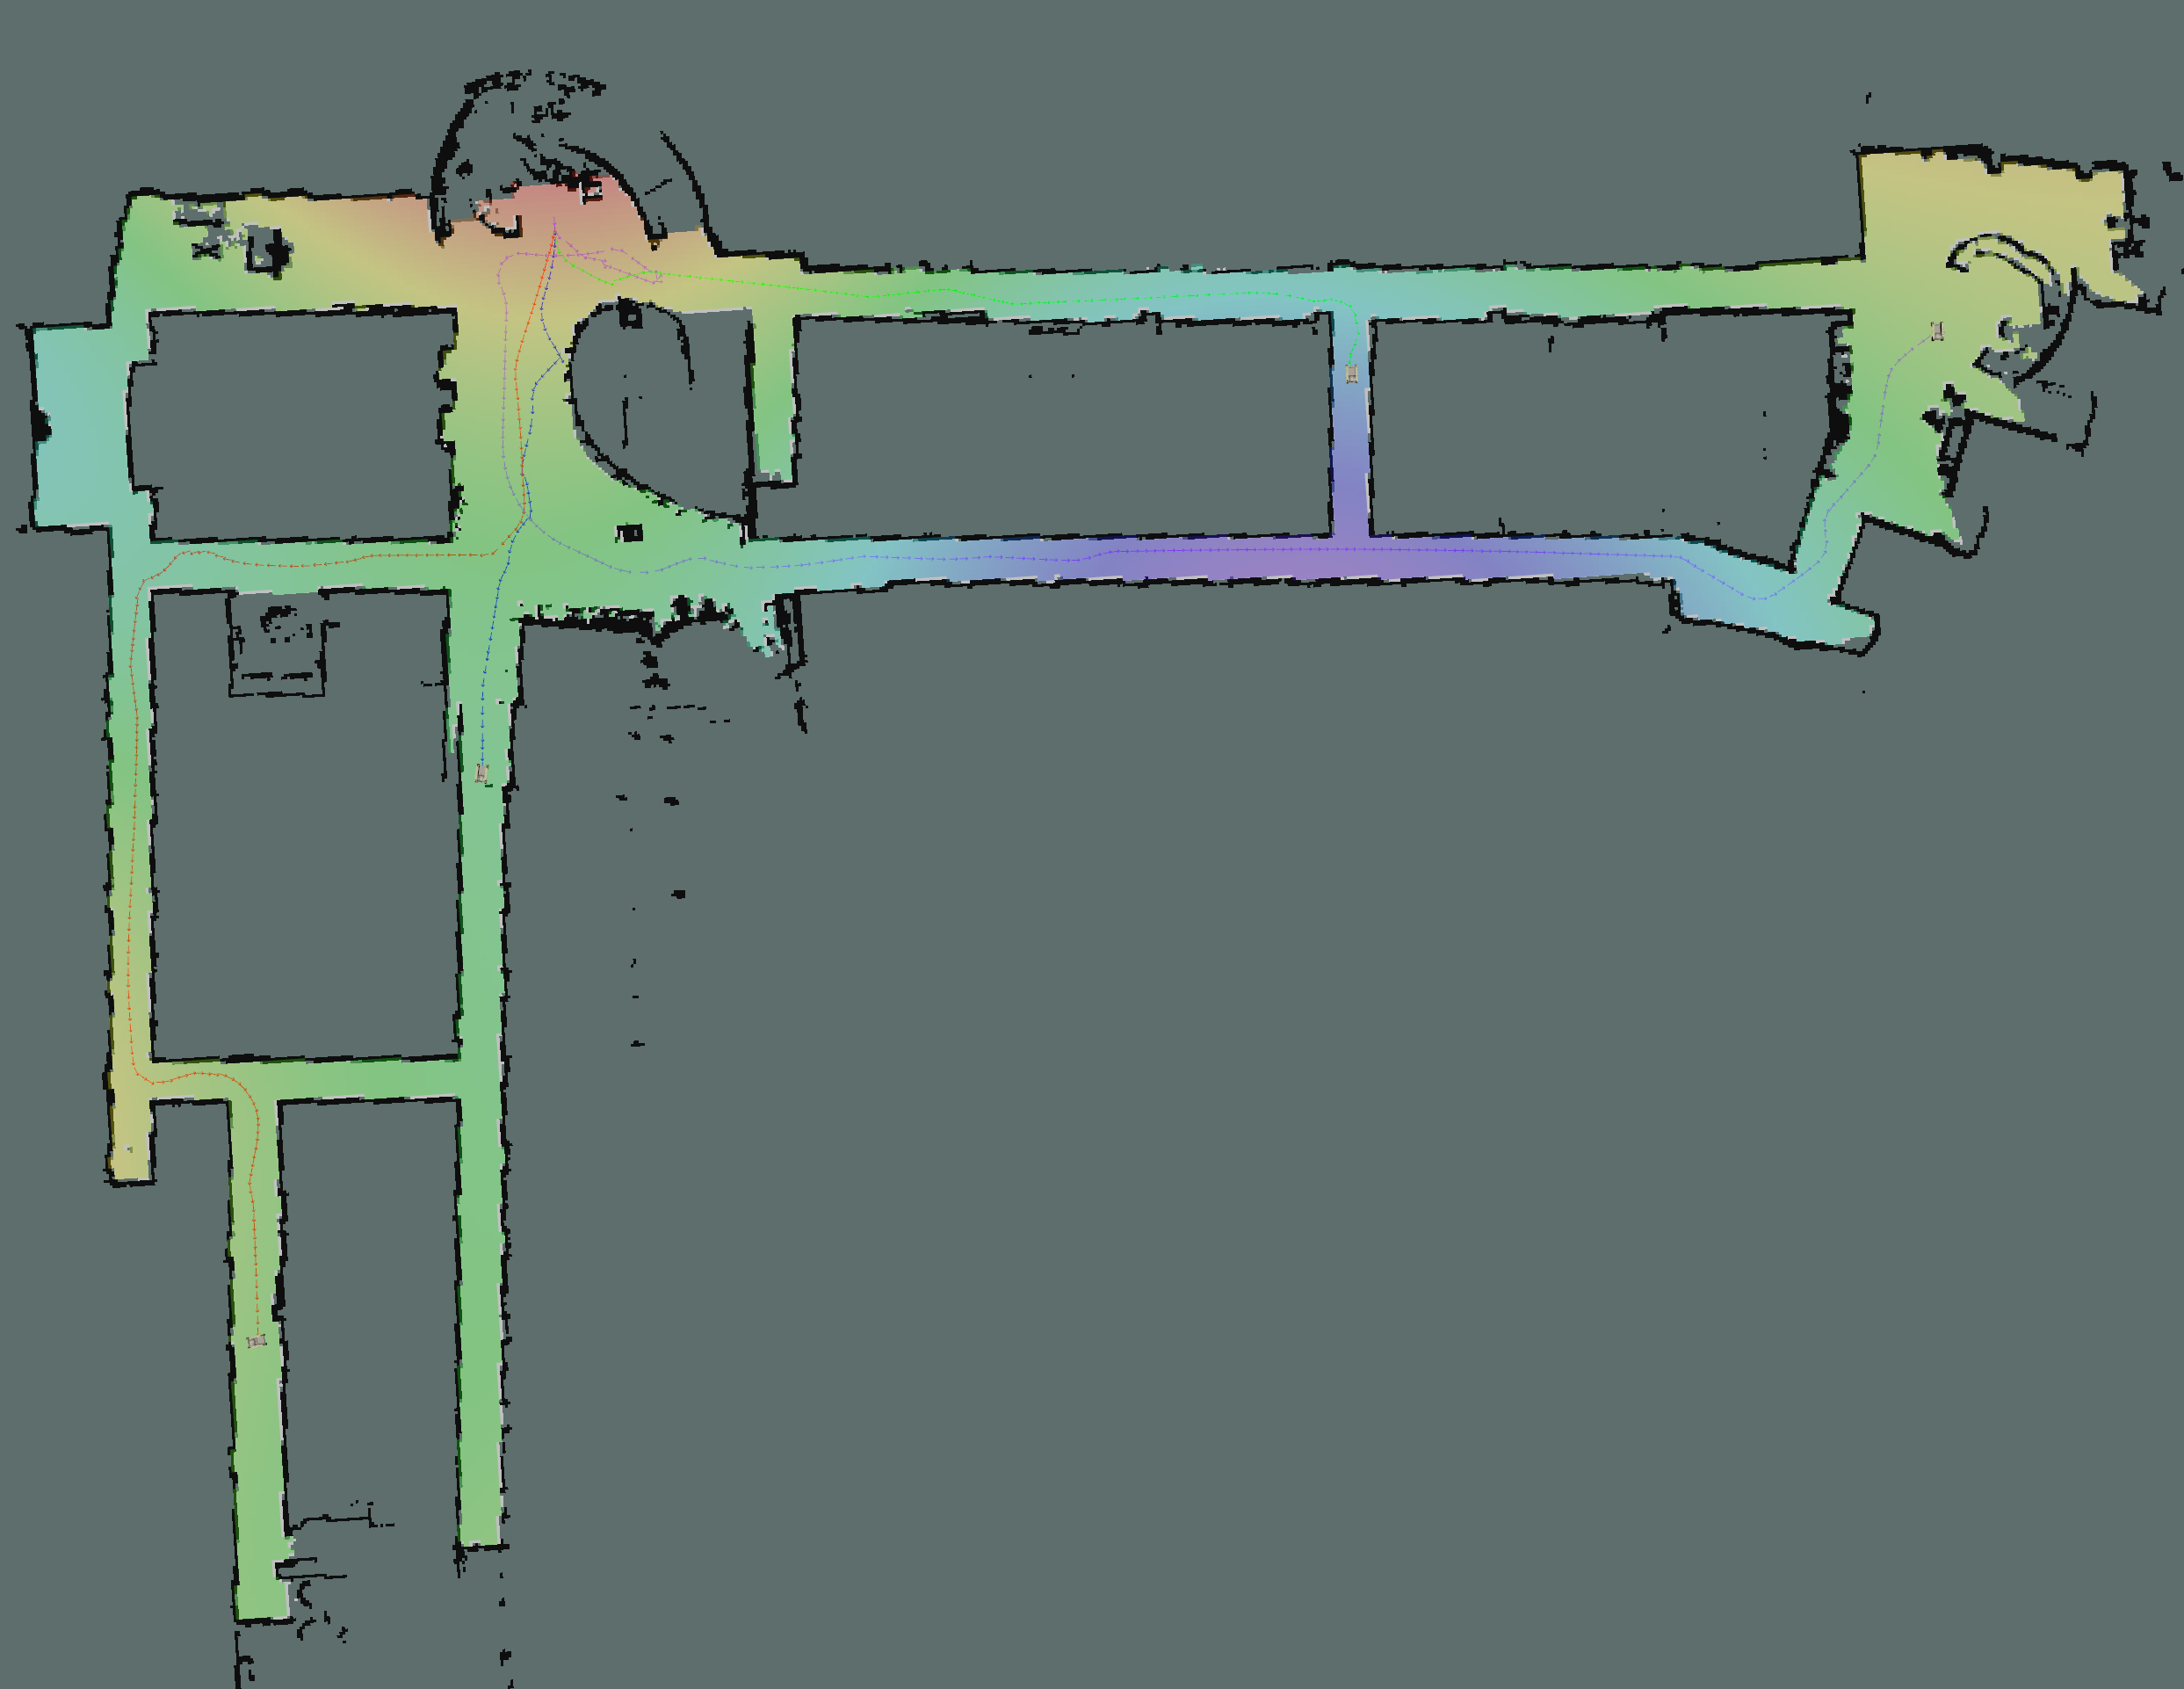
\includegraphics[width=.48\linewidth]{paper/files/media/multirobot_exp.png}%
  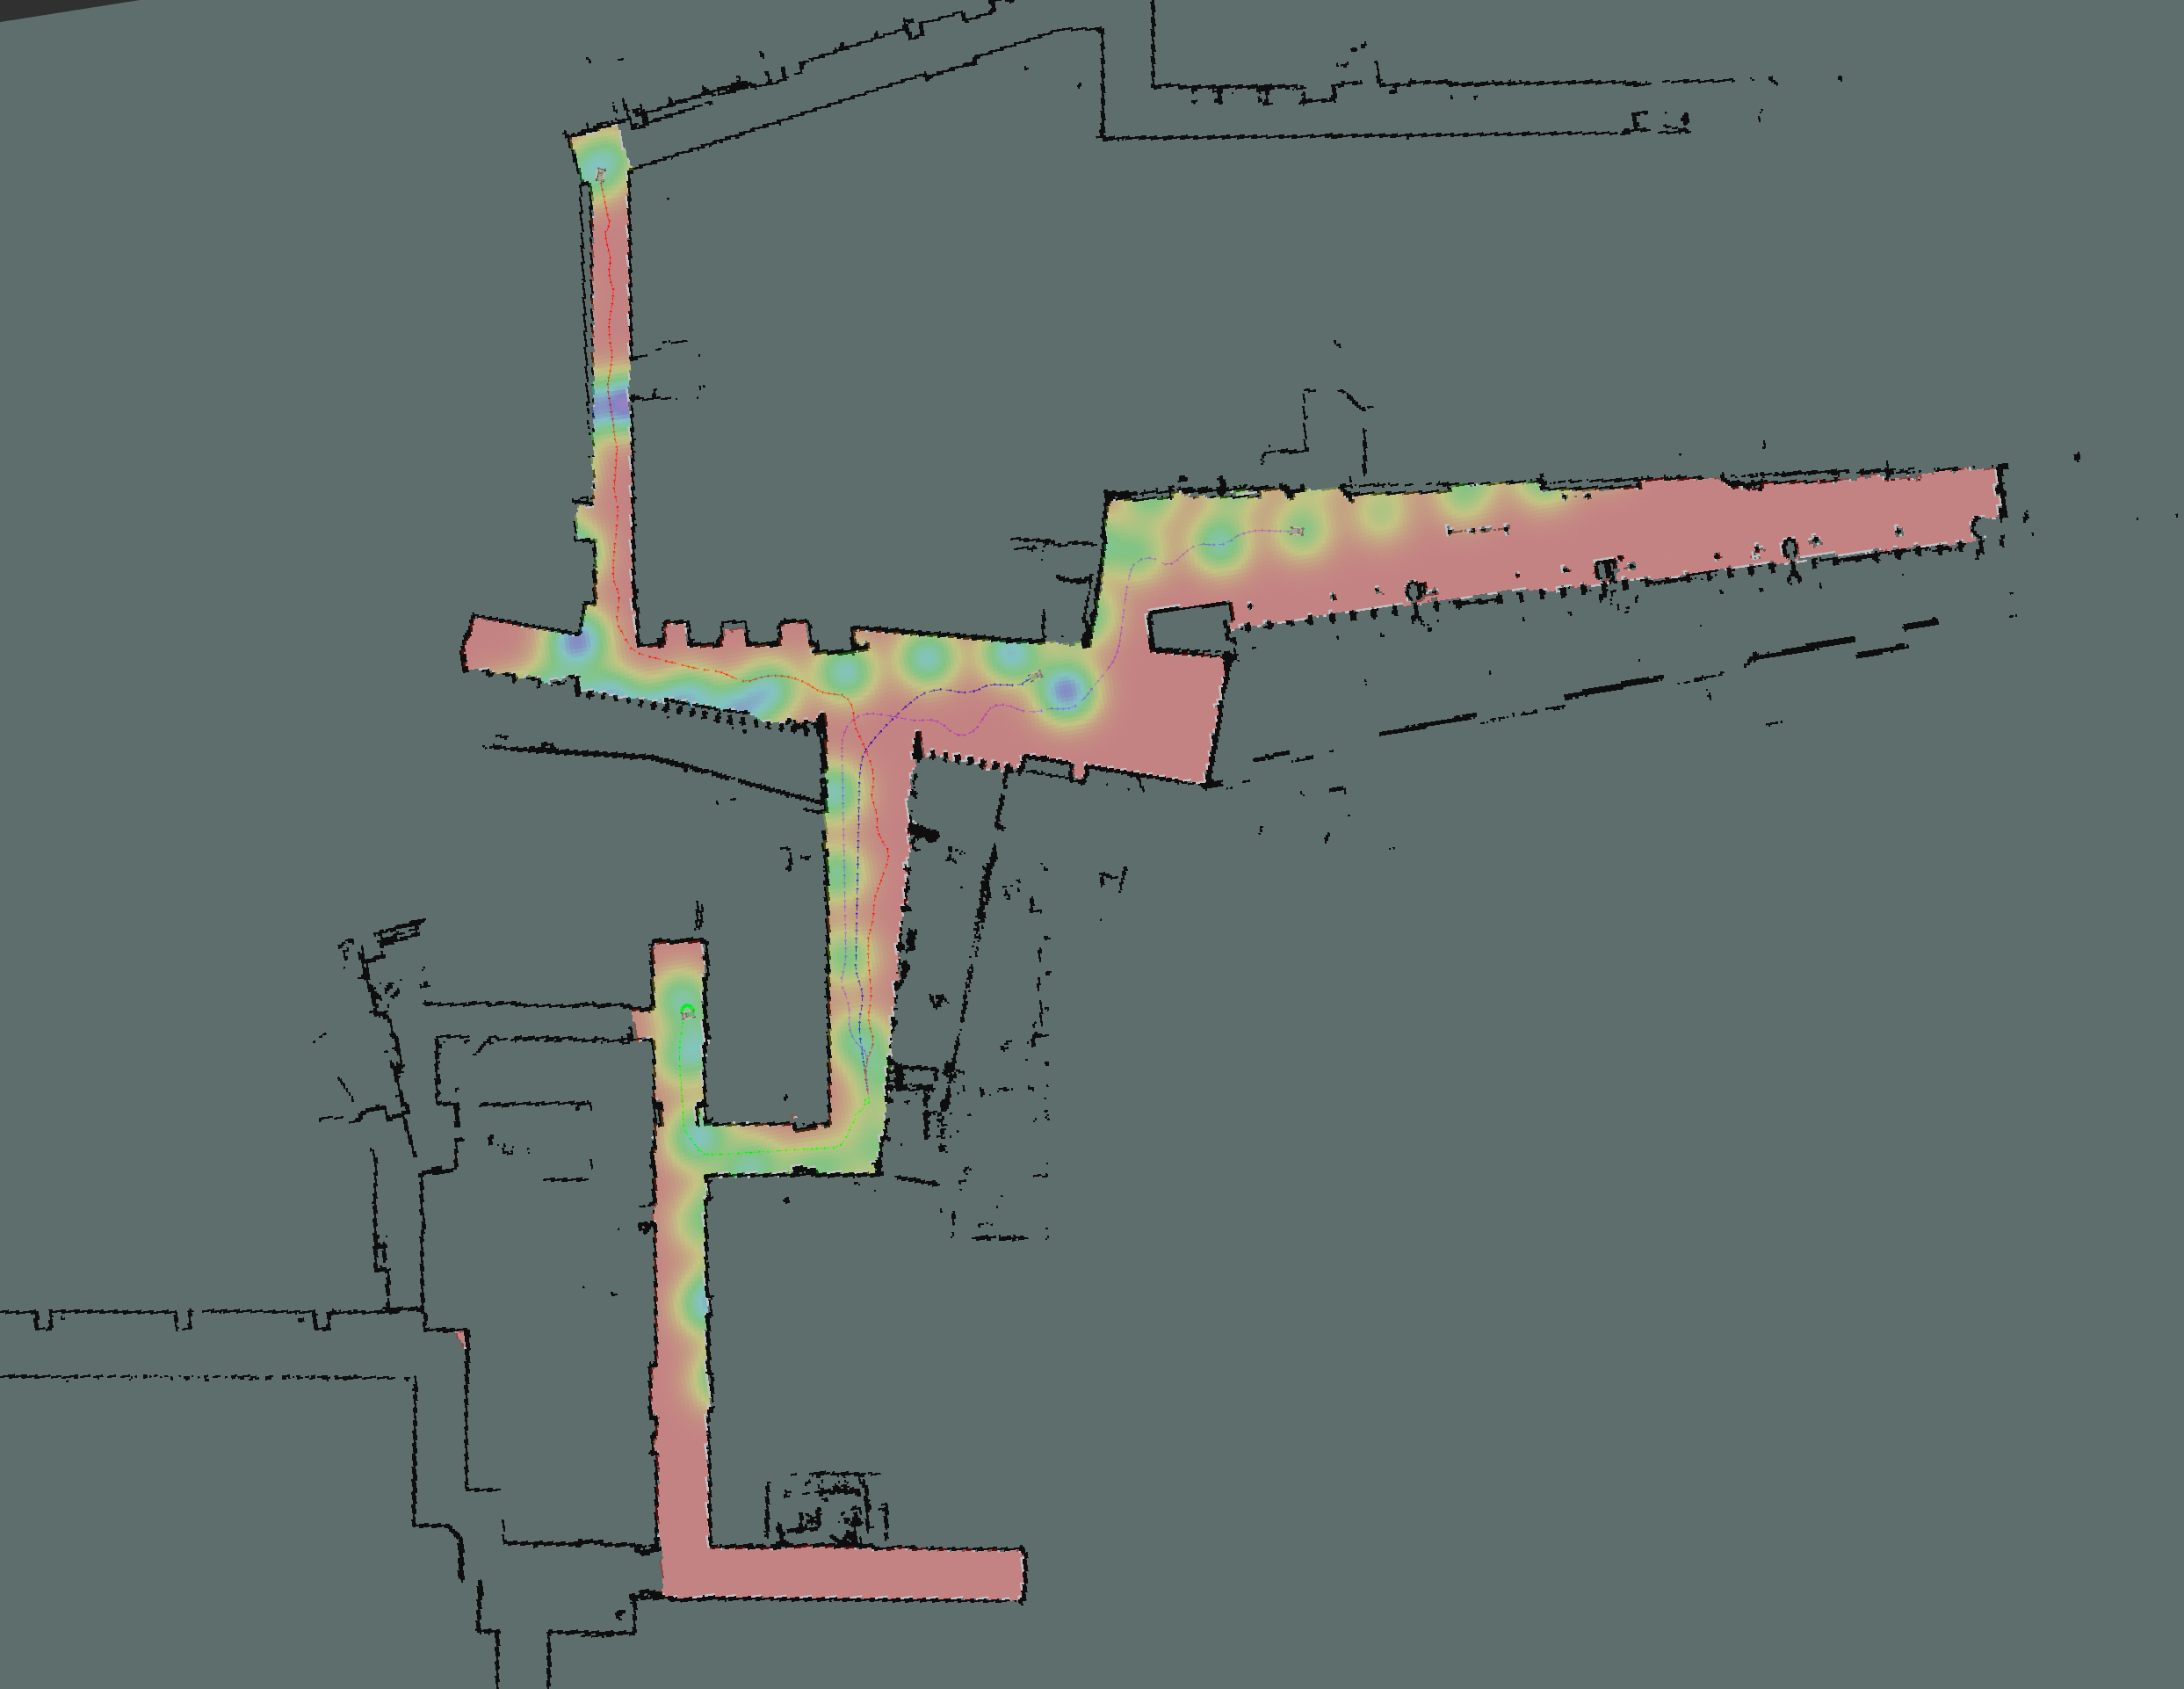
\includegraphics[width=.48\linewidth]{paper/files/media/multirobot_exp2.png}
 \caption{ Our multi-robot team exploring two different buildings on UC San Diego.. In color 
 graphics is shown the received signal strength indication (RSSI) and the trajectory of each robot.}
 \label{fig:multirobot-atk}
\end{figure*}
\section{Methodology}

We focus on a learning based approach. Our overall approach is shown in Fig.~\ref{fig:architecture}.


\subsection{Bayes Filter for SLAM}

We assume that our system is Markovian with the state vector $\state_t := [\map^\top,
\pose_t^\top, \act_{1,t}^\top, \tgt_1^\top, \dots \act_{N,t}^\top, \tgt_N^\top]^\top$, that includes map, robot
pose and the target poses.
However, only activation state $\act_{i,t}$, the lidar observation $\lidar_t$ and the signal $\rssi_t$ is observable.
To estimate the state, we use a typical Simultaneous Localization and
Mapping (SLAM) pipeline that uses Bayes Filter to update the distribution over the
state,
%
\begin{align}
  \bel_0(\state_0) &:= p(\state_0)
  \\
\bel_t(\state_{t}) &:= p(\state_t|\lidar_{1:t}, \rssi_{1:t}, \act_{1:N,1:t}, \ctrl_{1:t-1})
  \\
  \bel_t(\state_{t}) &\propto \E_{\state_{t-1}} \left[p(\lidar_{t}|\state_{t})p(\rssi_{t}| \state_{t})p(\state_{t}|\state_{t-1}, \ctrl_{t-1}) \right]
                       \label{eq:bayes-filter}
\end{align}%
% 

Here $p(\lidar_t|\state_{t})$, $p(\rssi_t|\state_t)$  and
$p(\state_t|\state_{t-1}, \ctrl_{t-1})$ are the lidar observation model
$\LidarModel$, signal $\RSSIModel$ and the state transition model.
The observation models are known,
%
\begin{align}
  \lidar_t | \state_t &\sim \N(\LidarModel(\pose_t, \map), \lCov)
  \\
  \rssi_t | \state_t &\sim \N\left(\sum_{i=1}^N \act_{i,t}\RSSIModel(\pose_t, \tgt_i, \map), \rCov\right).
\end{align}%
% 

The transition model for robot pose and the source activations is known,
%
\begin{align}
p(\state_t|\state_{t-1}, \ctrl_{t-1}) &= p(\pose_t|\pose_{t-1}, \ctrl_{t-1}, \map)\prod_{i=1}^N p(\act_{i,t}|\act_{i,t-1}, \pose_{t-1}, \tgt_i, \map)
  \\
 \pose_t|\pose_{t-1}, \ctrl_{t-1}, \map &\sim \N\left(\dyn(\pose_{t-1}, \ctrl_{t-1}, \map), \pCov \right)
  \\
  p(\act_{i,t}|\act_{i,t-1}, &\pose_{t-1}, \tgt_i, \map) \nonumber \\
                              &= \ind[\act_{i,t} = \max\{\AlgObjDet(\pose_{t-1}, \tgt_i, \map), \act_{i,t-1} \}],
\end{align}%
%
where $\act_{i,t}$ is observed deterministically.

As a result, our SLAM pipeline gives us beliefs over map $\bel_t(\map)$, robot
pose $\bel_t(\pose_t)$ and signal source locations $\bel_t(\tgt_i)$. We
represent $\bel_t(\map)$ as occupancy grid map $\bel_t(\map) \in [0,1]^{w \times
  h}$,
and robot pose and source locations as Gaussian distributions $\bel_t(\pose_t)
\sim \N(\mpose_t, \SPose_t)$ and $\bel_t(\tgt_i) \sim \N(\mtgt_{i,t}, \STgt_{i,t})$.


\subsection{Map prediction using image inpainting}

Having computed the distributions over map, robot pose and signal sources, we
want to compute the best action that leads to largest gain in information about
the signal sources.
To evaluate the cost of proposed actions, we need to know the map.
At any timestep large parts of the map may still be unknown.
We know that many environments, like urban indoor environments, exhibit
structured patterns forming priors over the maps.
To exploit these priors over certain environment types, we formulate the
map-prediction problem as image in-painting problem.
%
\begin{problem}[Map prediction as Image inpainting]
Given a map belief $\bel(\map) \in [0, 1]^{w \times h}$ and a mask $\mask \in
\{0, 1\}^{w \times h}$ such that the pixels $(i,j)$ where $\mask[i, j] = 0$ the
$\bel(\map[i, j])$ is assumed to be known while all other pixels are considered
unknown and need to be estimated. We assume a dataset of i.i.d. sampled maps and
masks $\Data = \{\bel_i(\map_i), \mask_i\}_{i=1}^d$ is given. We train a
parameteric estimator of the desired output $\bel'(\map)$ given the masked map $\bel(\map[\mask])$,
%
\begin{align}
  \Theta &= \arg\max_{\Theta} \sum_{i \in \Data} \log p (\bel_i(\map_i)| \bel_i(\map_i[\mask_i]); \Theta),
\end{align}%
% 
where $\bel_i(\map_i[\mask_i])$ denotes a masked map where only the pixels
$bel_i(\map_i[k,l])$ where $\mask_i[k,l] = 0$ are retained and the rest are set
to 0.
\end{problem}

A lot of work has been done image in-painting domain, we use a well written,
easy to run library called DeepFill~\cite{yu2018DeepFill} for map-prediction.
We briefly explain the DeepFill algorithm for sake of completeness.

\subsubsection{Image inpainting with DeepFill}

The architecture diagram for DeepFill is shown in Fig~\ref{fig:deepfill}.
DeepFill algorithm is based on Generative Adversarial Networks
(GAN)~\cite{goodfellow2014GAN} which are models to generate realistic images.
The main idea for GAN is a pair of adversarial networks, a Generator $G(b;
\theta_g)$ and a discriminator $D(a; \theta_d)$.
Given samples of real images $a \sim p_{\text{data}}(a)$, and images generated by
generator $G(a; \theta_g)$, we want to train the discriminator $D(a; \theta_d)$
to distinguish between real and fake images. Thus the GANs are trained with the
following loss function~\cite{goodfellow2014GAN},
%
\begin{align}
  \theta^*_g, \theta^*_d = \min_{\theta_g} \max_{\theta_d} \E_{a \sim p_{\text{data}}(a)}[\log D(a)]
  + \nonumber \\  \E_{b \sim p_z(b)} [\log(1-D(G(b))]
\end{align}%
% 

While the detailed architecture of DeepFill algorithm is beyond the scope of this
paper, we mention the main idea of \textit{Gated convolutions}. Gated convolutions learn a
learned gate from the mask that gets applied to the regular feature convolutions
from the image~\cite{yu2018DeepFill},

%
\begin{align}
  \textit{Gating}_{y,x} &=  W_g \circledast I 
  \\
  \textit{Feature}_{y,x} &=  W_f \circledast I 
  \\
  O_{y,x} &= \phi(\textit{Feature}_{y,x}) \otimes \sigma(\textit{Gating}_{y,x}),
\end{align}%
% 
where $\circledast$ is the convolution operator, $\sigma$ is sigmoid function,
$\phi$ is any non-linear activation and $\otimes$ is element-wise product.


% 
\subsection{Active exploration in partially observable  environments}

We use ideas from information adaptive sampling~\cite{choudhury2017adaptive},
to compute the optimal trajectory for maximum information gain. However, unlike
Choudhury~et~al.~\cite{choudhury2017adaptive} we use a model-based learning
algorithm instead of model-free imitation-learning.
Specifically, having a model for predicting missing parts of the map.
We use the predicted map to convert the \texttt{Unkown-Map} information
gathering problem into a \texttt{Known-Map} information gathering problem.



\section{Experiments}

\subsection{Map prediction}

The first step in making better decisions about the future is to predict the future.
We learn the prior of over indoor environments and use it to predict the unknown
parts in the map. Some of the examples of inputs, mask and predicted pairs are
given in Figure~\ref{fig:map-prediction}.

\subsubsection{Generation of training data}

We collect indoor maps from various datasets ~\cite{howard2003radish}.
We run an occupancy grid algorithm, specifically Omnimapper~\cite{Trevor14ICRA} and generate maps. 
The maps are saved and a mask is generated by running morphological operations
on the known part of the map.
The newly explored known part of the maps is masked out and the map and mask
pair are fed into the image-inpainting training algorithm.
The image-inpainting algorithm is only fine-tuned on this new dataset.
The result of map-prediction is shown in Figure~\ref{fig:map-prediction}.


\subsection{Real World Experiments}

We evaluate our system performing a series of experiments incorporated real-world robot operation within environments over Atkinson and Jacobs Halls on the campus of the University of California, San Diego.  This large environments contains obstacles that are typical of office buildings.

Each robot generates their own map using our mapping framework OmniMapper~\cite{Trevor14ICRA}. An initial pose estimate is used to speed up the convergence of the localization routine. While the localization routine is converged on a pose hypothesis, the corresponding RSSI measurements are computed into a GP model using  libGP~\cite{BlumLibGP}. 

We model RSSI using Gaussian Process (GP) regression, a standard method for spatial field modeling~\cite{Rasmussen2006}.
The GP approximates measurements at different locations with Gaussian functions based on a prior mean and covariance function $k(\cdot,\cdot)$, also known as the kernel.
When a sample $y$ at location ${\bf x}$ is added to the GP, the Gaussians at locations ${\bf x}'$ are updated based on the chosen kernel, where ${\bf x,x}' \in \mathbb{R}^2$.

For each possible sampling location ${\bf x}_*$ the GP has a predictive mean and predictive variance~\cite{Rasmussen2006}:

\begin{align}
 \mu_{y_*}({\bf x}, {\bf x}_*, y) &=  k({\bf x}_*,{\bf x}) k({\bf x},{\bf x}) y\\
 \sigma^2_{y_*}({\bf x}, {\bf x}_*) &= k({\bf x}_*,{\bf x}_*) - k({\bf x}_*,{\bf x}) k({\bf x},{\bf x})^{-1} k({\bf x},{\bf x}_*)
\end{align}
% 
where ${\bf x}$ and $y$ are training locations and measurements, ${\bf x_*}$ are test locations,
and $k(\cdot,\cdot)$ is the kernel, i.e. the covariance function. The predictive variance is especially useful in adaptive sampling, because it gives an estimate of the confidence in the predicted mean, and robots can choose to sample in locations with high model uncertainty.


\section{Conclusion}
We present a method for stochastic seeking in partially observable environments. 
We provide a method to  predict unseen portions of the map using image inpainting algorithms.
This allows us to compute information gain in the unseen parts of the map and hence plan efficiently for maximum information gain.


%%%%%%%%%%%%%%%%%%%%%%%%%%%%%%%%%%%%%%%%%%%%%%%%%%%%%%%%%%%%%%%%%%%%%%%%%%%%%%%%%%%%%%%%%%%%%%%%%%%%%%%%%
%% bibliography: see CFP for number of permitted pages

\bibliographystyle{ACM-Reference-Format}  % do not change this line!
\def\localbib{\string~/wrk/group-bib/shared}
\IfFileExists{\localbib.bib}{
\bibliography{\localbib,sources}}{
\bibliography{sources}}


%\input{files/appendix.tex}

\end{document}